\documentclass[a4paper,12pt]{article}
\usepackage{amsmath, empheq, graphicx, hyperref, physics, siunitx}
\usepackage[section]{placeins}
\usepackage[extrafootnotefeatures]{xepersian}
\settextfont{XB Zar}
\title{پروژه فصل 2 مکانیک تحلیلی 1}
\author{صالح شاملو، ارمیا اعتمادی}
\date{2 آبان 1399}

\hypersetup{
	colorlinks=true,
	linkcolor=red,
	filecolor=magenta,
	urlcolor=blue
}

\begin{document}
	\maketitle
	\begin{abstract}
		یک تقریب برای نیروی مقاومت هوا در برابر حرکت یک جسم در یک سیال به شکل زیر است:
		\begin{equation}
			f = \frac{1}{2}C_w \rho A v^2
		\end{equation}
		که $v$ سرعت جسم، $\rho$ چگالی سیال، $A$ سطح مقطع عمود بر جهت سرعت و $C_w$ ثابتی وابسته به شکل جسم است.
		در سرعت‌های نزدیک به سرعت صوت و بیشتر از آن، مقدار $C_w$ ثابت نیست. در این نوشته حرکت یک پرتابه با سرعت مافوق صوت را با استفاده از روش‌های عددی بررسی می‌کنیم.
	\end{abstract}
	\newpage
	\section{تقریب ضریب $C_w$}
	در کتاب \emph{دینامیک کلاسیک ذرات و سیستم‌ها}\LTRfootnote{Classical Dynamics of Particles and Systems} نمودار تقریبی $C_w$ برحسب سرعت برای یک گلوله داده شده.
	از نموداری مشابه استفاده می‌کنیم.
	\begin{figure}[h]
		\centering
		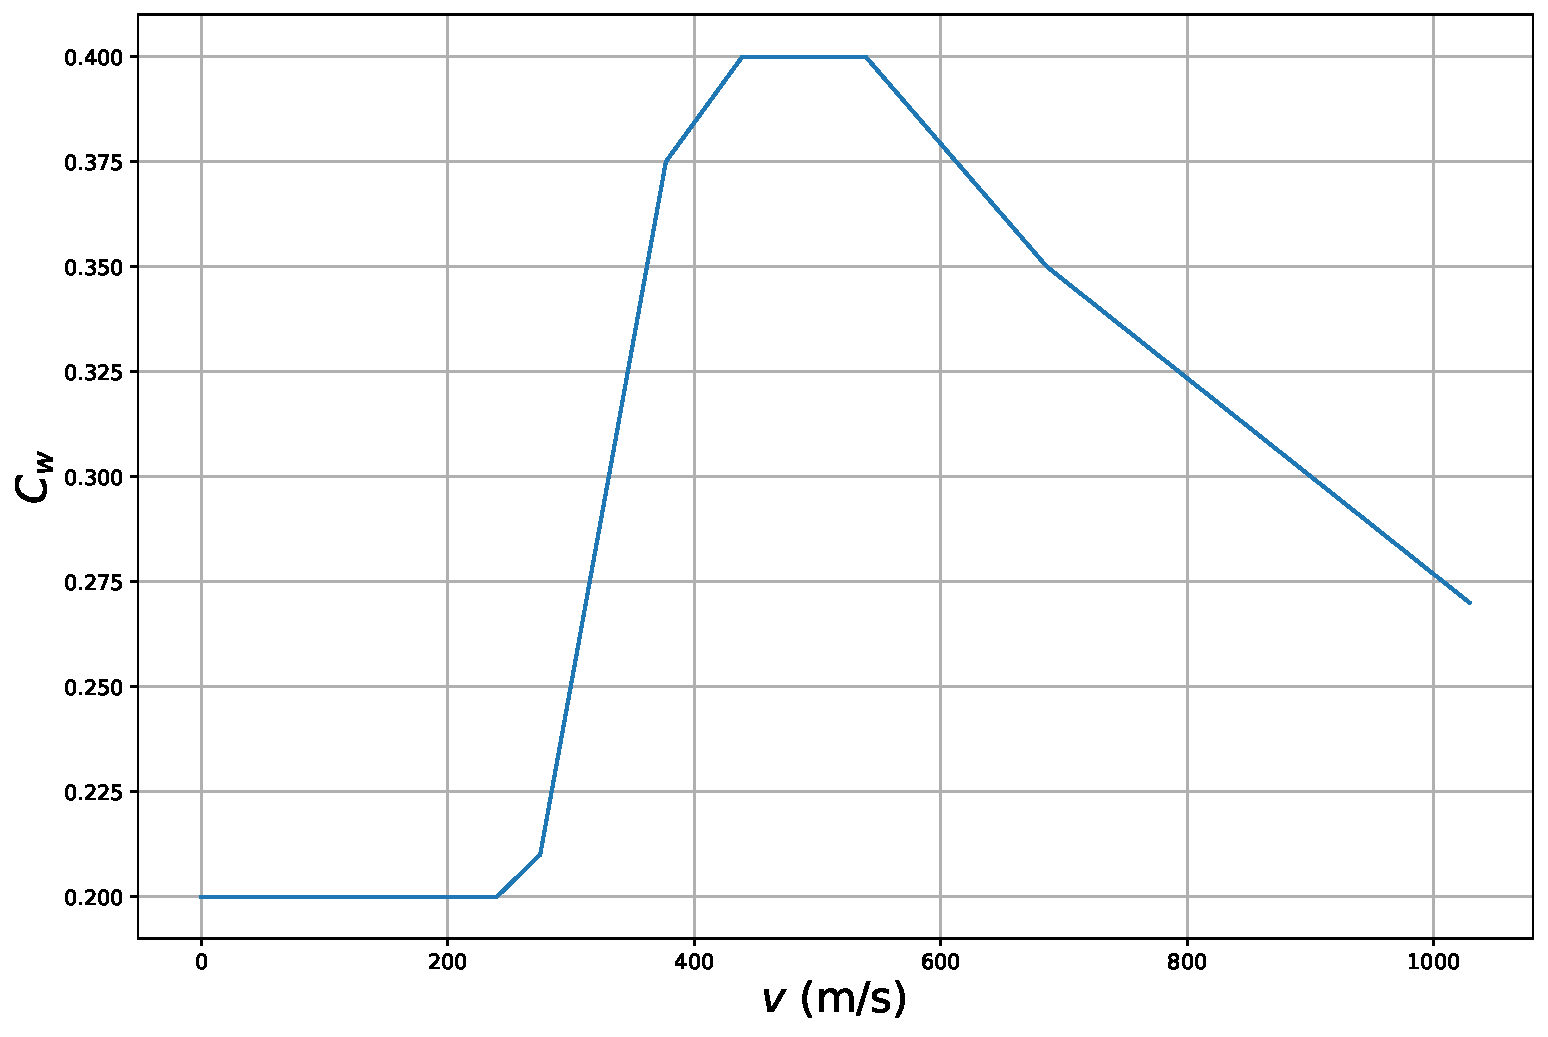
\includegraphics[width=\linewidth]{../figures/Cw}
		\caption{تقریب $C_w$}
	\end{figure}
	\section{معادلات حرکت}
	\begin{align}
		\sum \vb{F} &= m\vb{a} \\
		\vb{F_g} + \vb{f} &= m\vb{a} \\
		m\vb{g} - \frac{1}{2}C_w \rho A v^2 \vu{v} &= m\vb{a}
	\end{align}
	\begin{empheq}[left=\empheqlbrace]{align}
		\ddot{x} &= -\frac{C_w \rho A}{2m}v\dot{x} \\ \notag \\
		\ddot{y} &= -\frac{C_w \rho A}{2m}v\dot{y} - g
	\end{empheq}
	با استفاده از روش رونگه-کوتا\LTRfootnote{Runge-Kutta} معادلات دیفرانسیل را به صورت عددی حل می‌کنیم.
	 
	تحلیل را برای یک گلوله با مقطع دایره به شعاع $\SI{10}{\centi\meter}$ انجام می‌دهیم. سه حالت را درنظر می‌گیریم:
	\begin{enumerate}
		\item بدون مقاومت هوا
		\item گلوله 30 کیلوگرمی (وزن تقریبی گلوله کروی فولادی با شعاع 10 سانتی‌متر) در مقاومت هوا
		\item گلوله 2 کیلوگرمی (وزن تقریبی گلوله کروی چوبی با شعاع 10 سانتی‌متر) در مقاومت هوا
	\end{enumerate}
	
	\section{مسیر حرکت پرتابه}
	\begin{figure}[h]
		\centering
		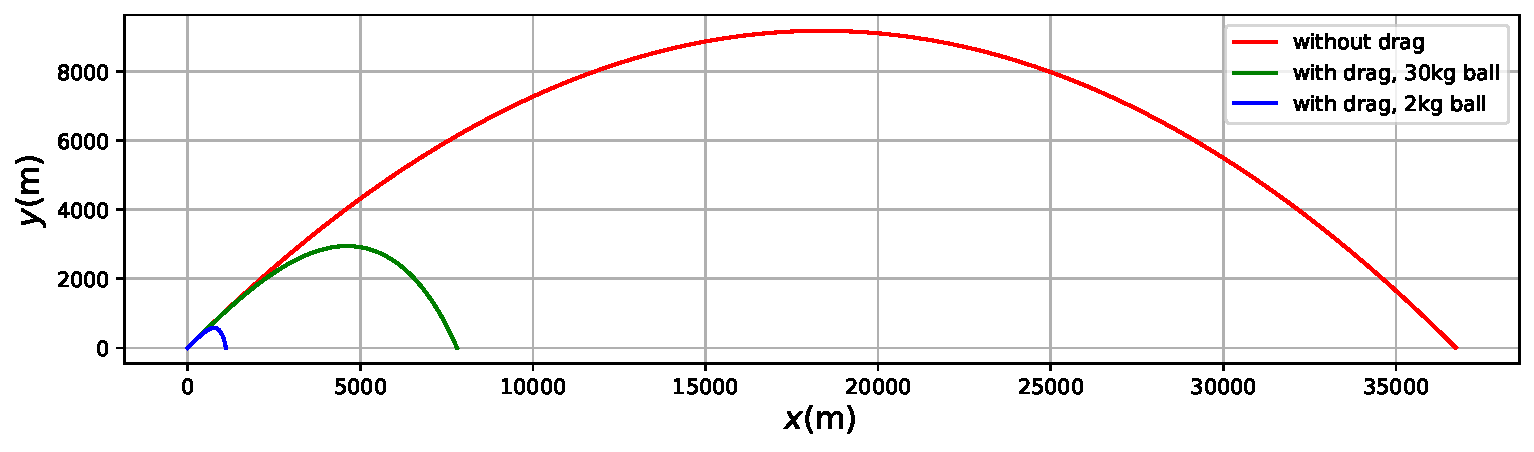
\includegraphics[width=\linewidth]{../figures/xy}
		\caption{مسیر حرکت پرتابه‌ها}
	\end{figure}
	\begin{figure}[h]
		\centering
		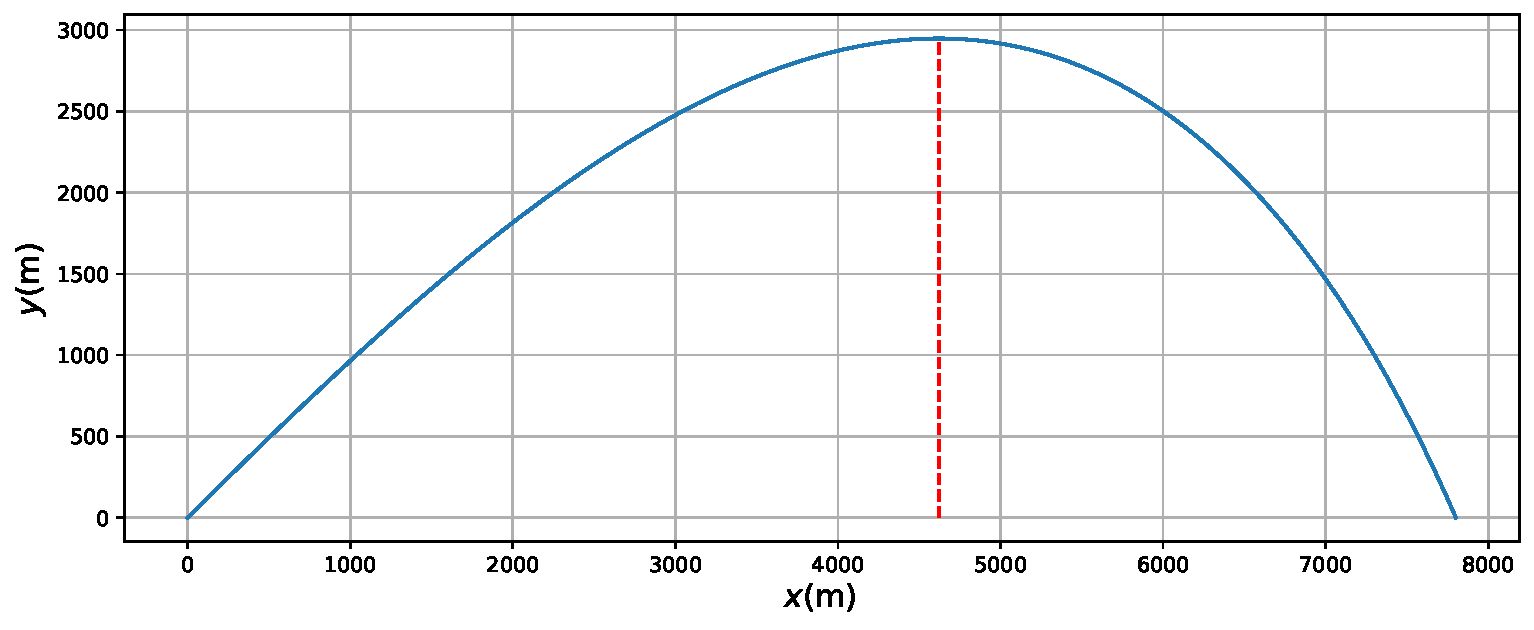
\includegraphics[width=\linewidth]{../figures/heavy}
		\caption{مسیر حرکت پرتابه 30 کیلوگرمی}
	\end{figure}
	\begin{figure}[h]
		\centering
		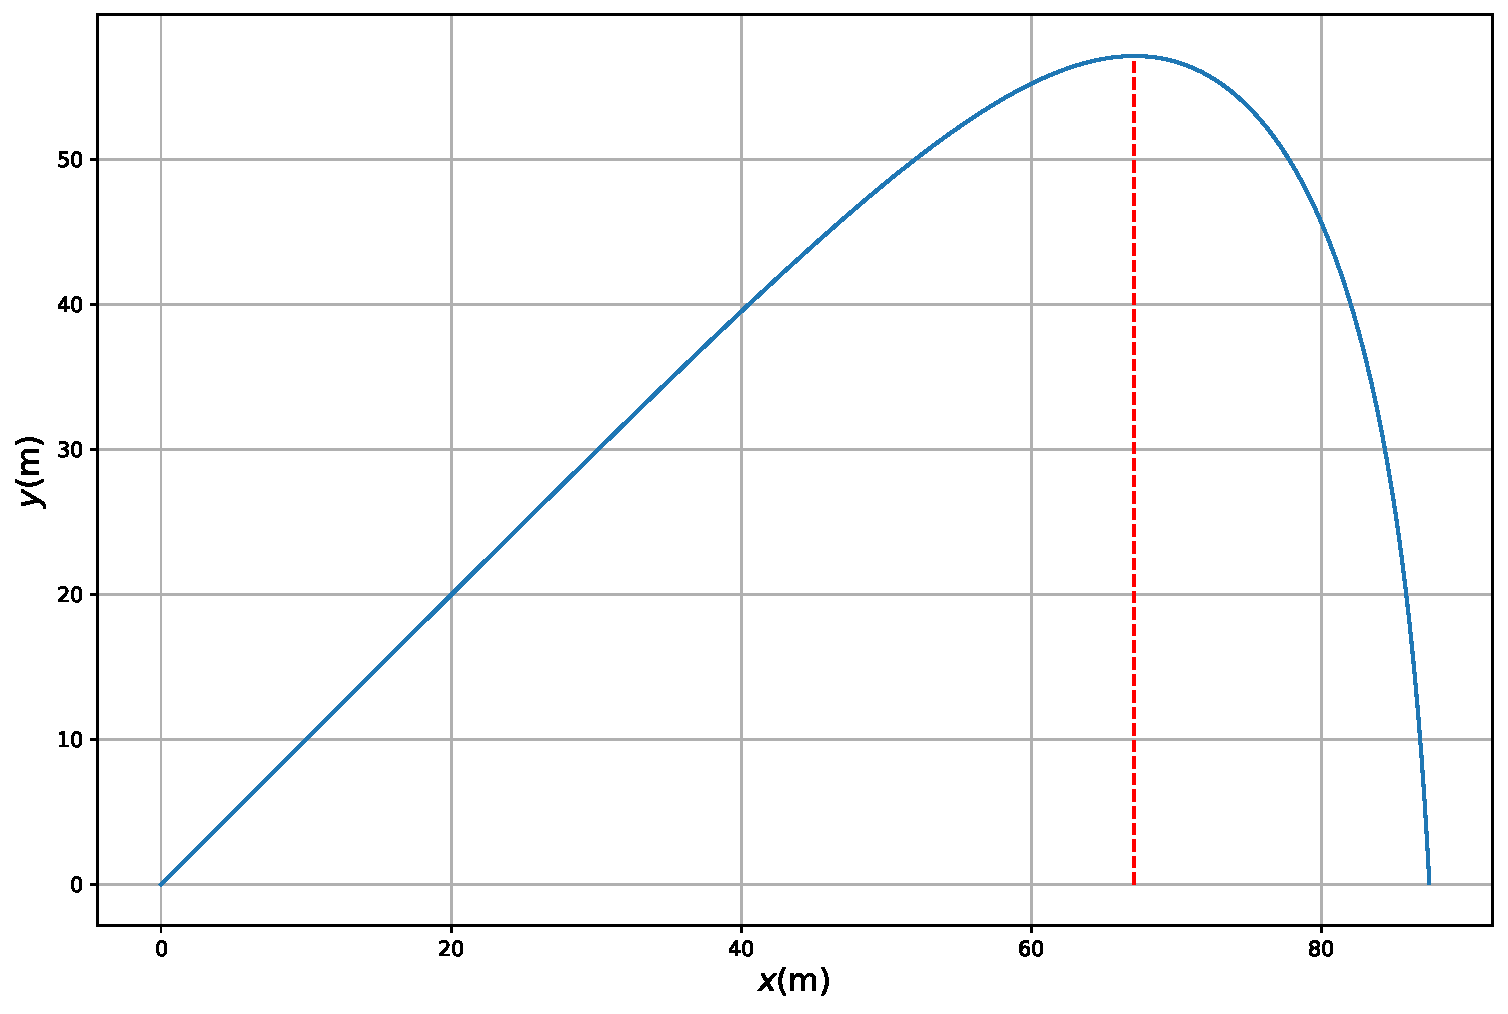
\includegraphics[width=\linewidth]{../figures/light}
		\caption{مسیر حرکت پرتابه‌ای 100 گرمی. در این نمودار اثرات مقاومت هوا راحت‌تر دیده می‌شود.}
	\end{figure}
	\subsection{بُرد}
	\begin{equation}
		\text{بدون مقاومت هوا}: R = \SI{36732}{\meter}
	\end{equation}
	\begin{empheq}[left={\text{با مقاومت هوا}\empheqlbrace}]{align}
		R_{30\mathrm{kg}} &= \SI{7801.1}{\meter} \\
		R_{2\mathrm{kg}} &= \SI{1107.7}{\meter}
	\end{empheq}
	\subsection{ارتفاع بیشینه}
	\begin{equation}
		\text{بدون مقاومت هوا}: H = \SI{9183.7}{\meter}
	\end{equation}
	\begin{empheq}[left={\text{با مقاومت هوا}\empheqlbrace}]{align}
		H_{30\mathrm{kg}} &= \SI{2948.1}{\meter} \\
		H_{2\mathrm{kg}} &= \SI{575.92}{\meter}
	\end{empheq}
	\subsection{زمان پرواز}
	\begin{equation}
		\text{بدون مقاومت هوا}: T = \SI{86.579}{\second}
	\end{equation}
	\begin{empheq}[left={\text{با مقاومت هوا}\empheqlbrace}]{align}
		T_{30\mathrm{kg}} &= \SI{47.965}{\second} \\
		T_{2\mathrm{kg}} &= \SI{21.122}{\second}
	\end{empheq}
	\newpage
	\section{$x(t), y(t)$}
	\begin{figure}
		\centering
		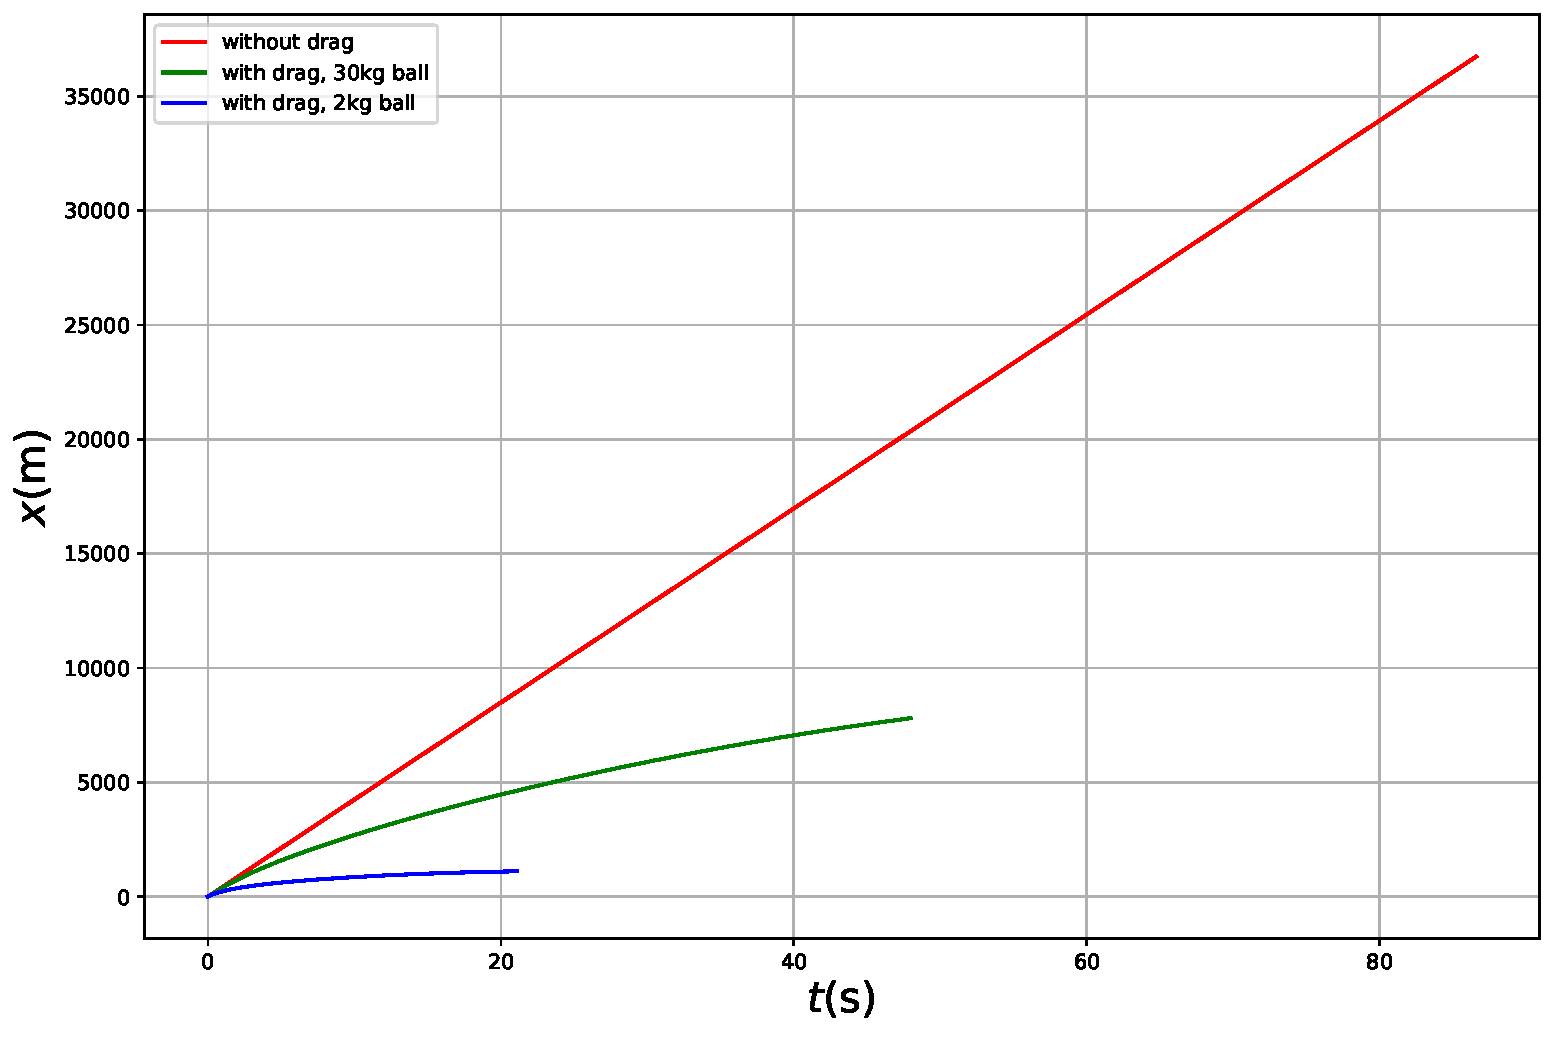
\includegraphics[width=\linewidth]{../figures/xplot}
		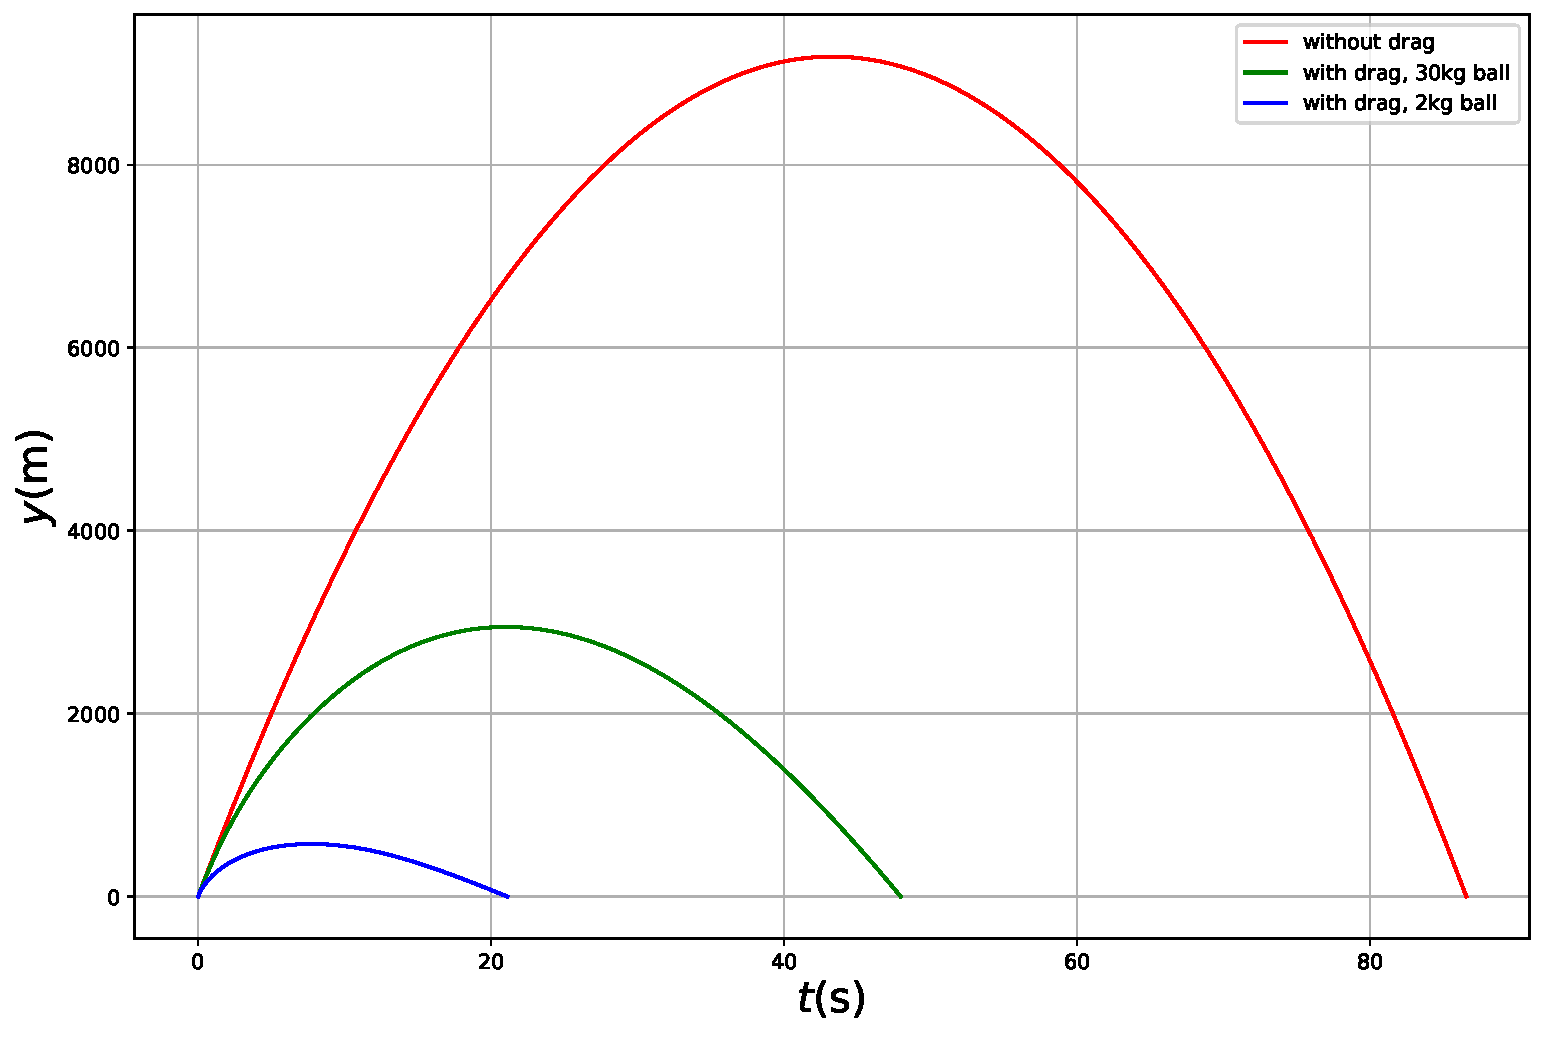
\includegraphics[width=\linewidth]{../figures/yplot}
	\end{figure}
	\newpage
	\section{$\dot{x}(t),\dot{y}(t)$}
	\begin{figure}[h]
		\centering
		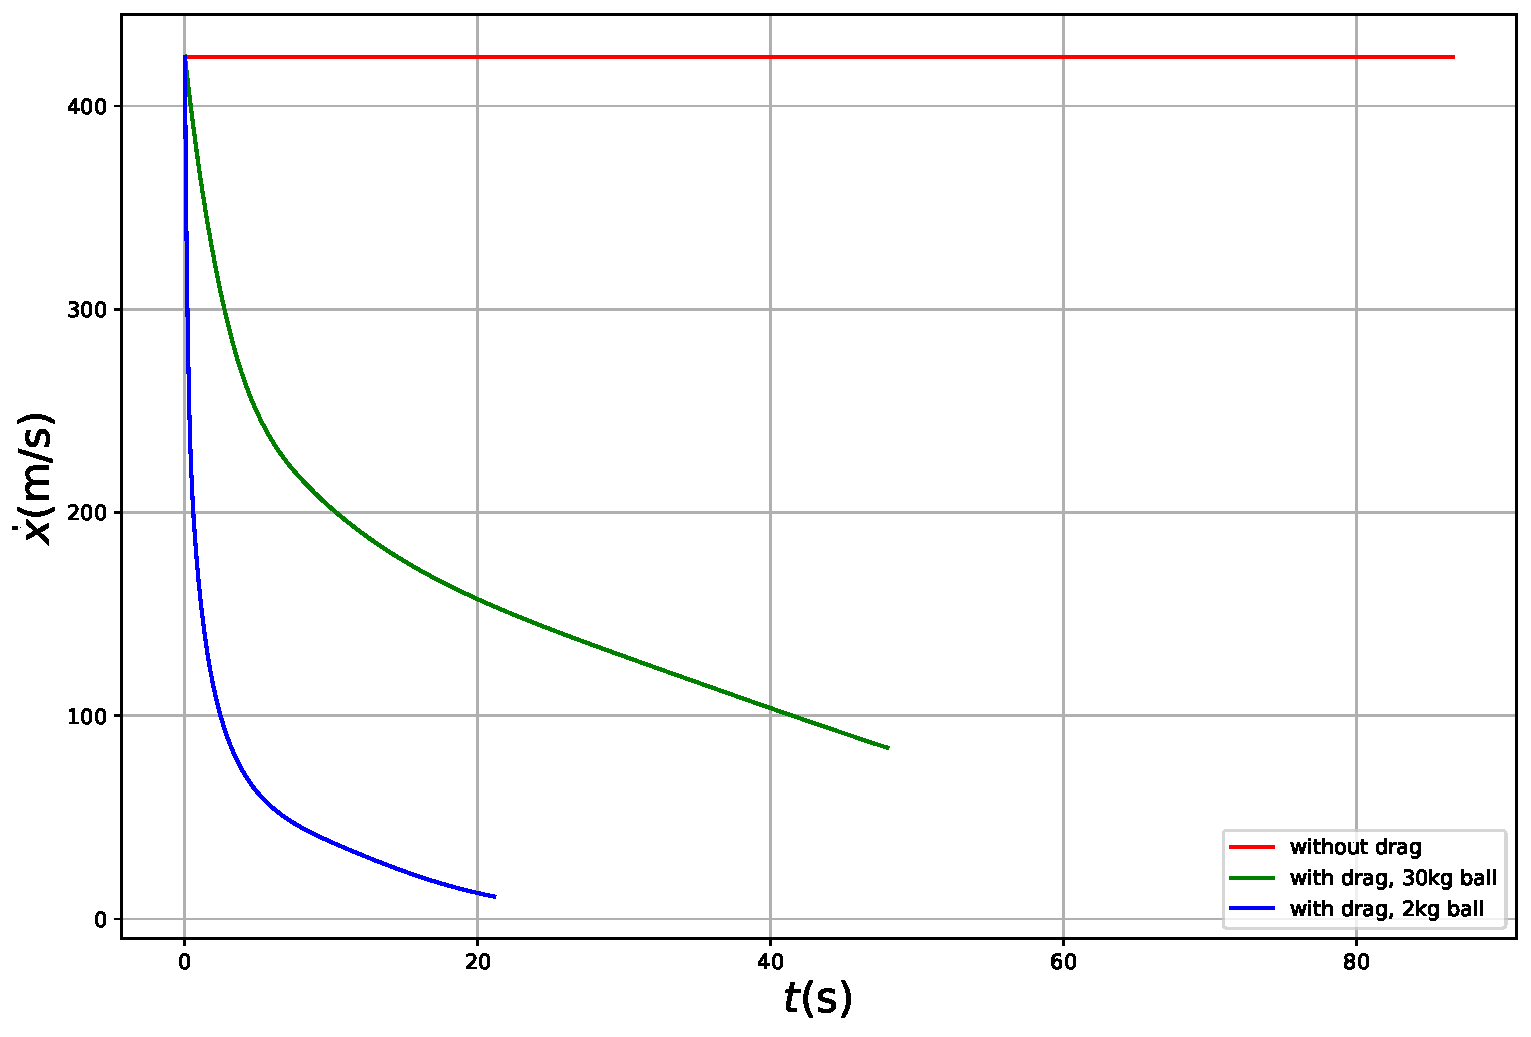
\includegraphics[width=0.874\linewidth]{../figures/vxplot}
		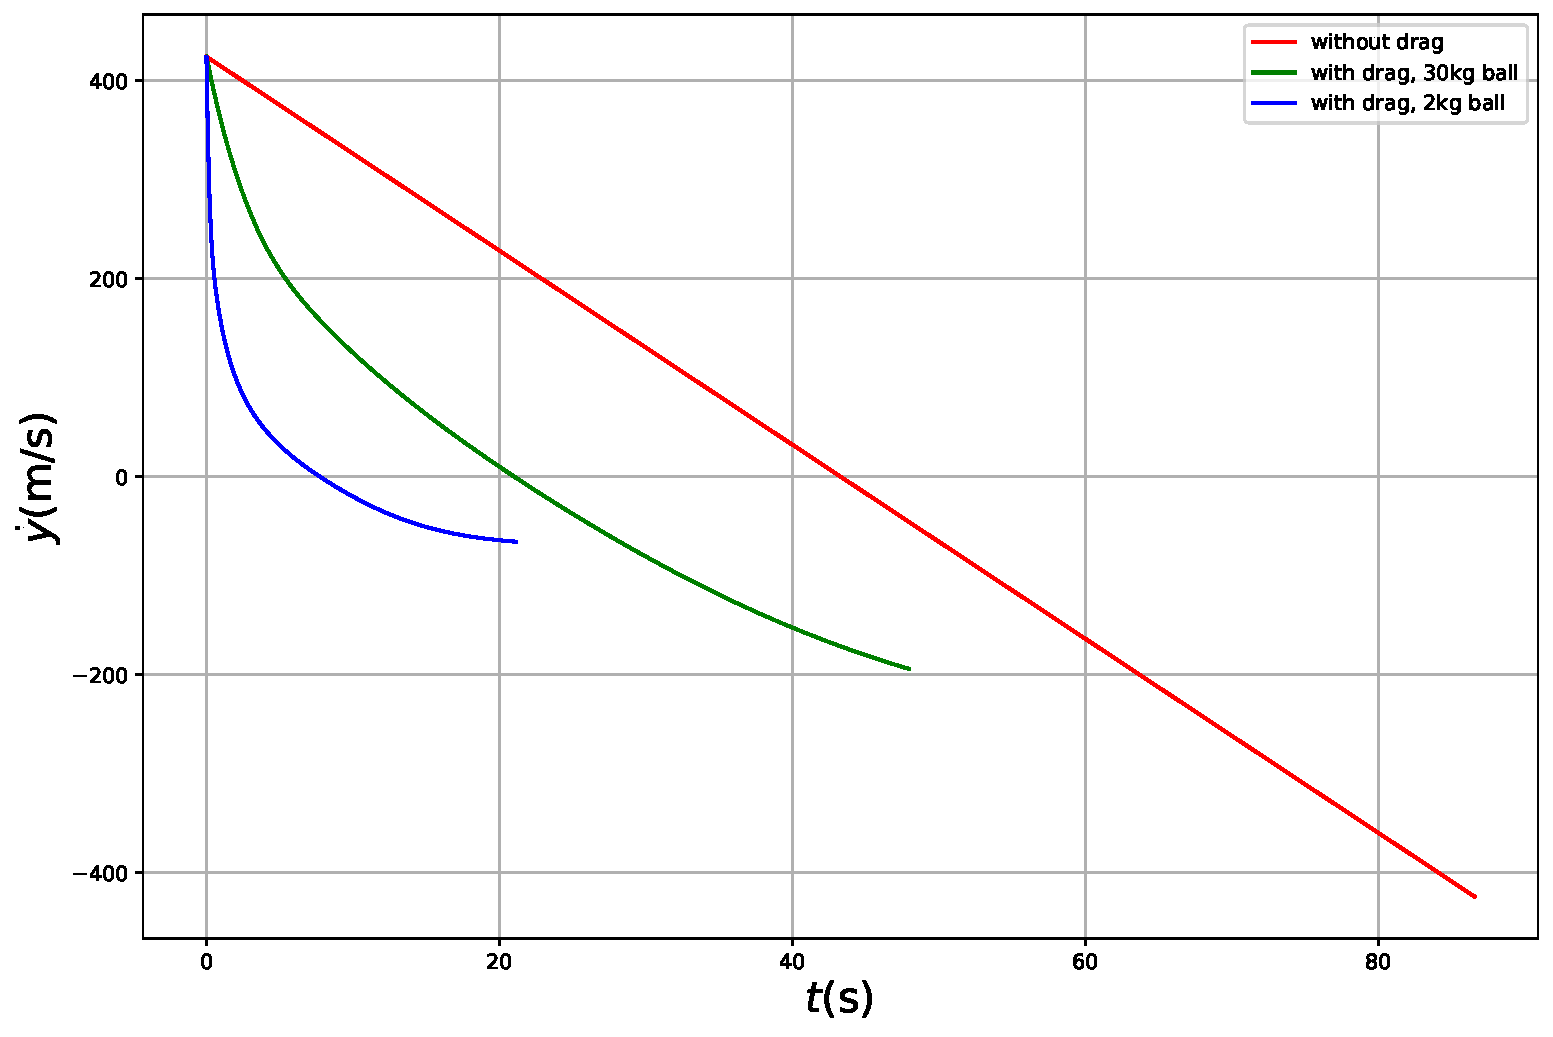
\includegraphics[width=0.874\linewidth]{../figures/vyplot}
	\end{figure}
	\newpage
	\section{$\dot{x}(x),\dot{y}(y)$}
	\begin{figure}[h]
		\centering
		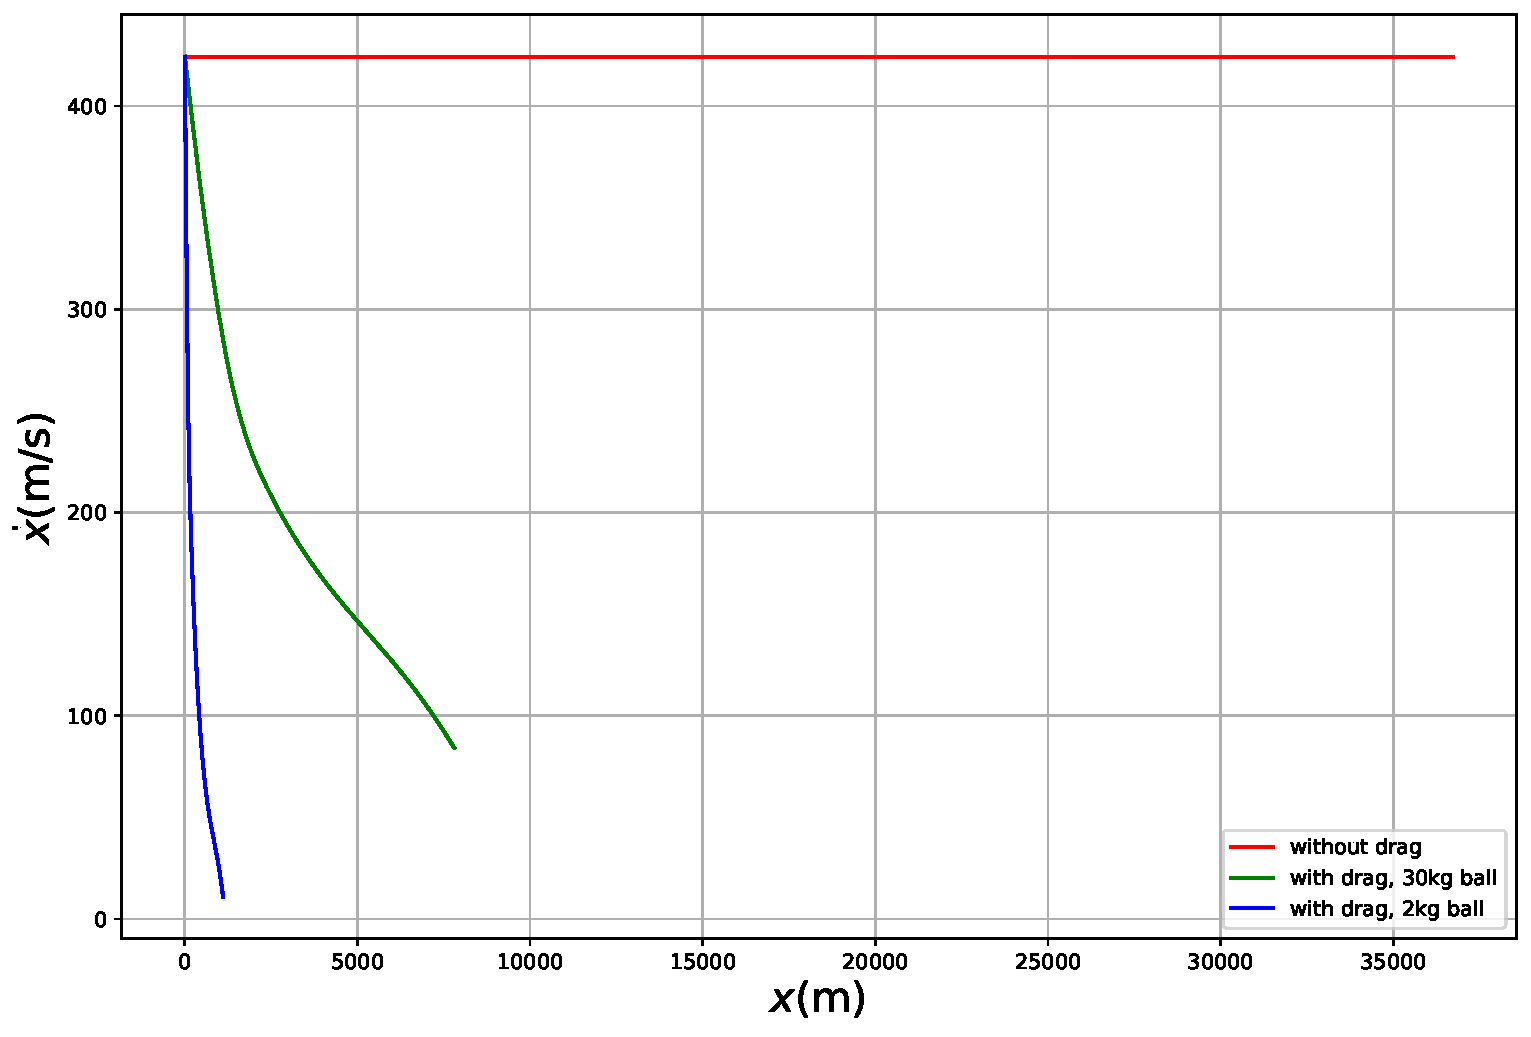
\includegraphics[width=0.87\linewidth]{../figures/xvx}
		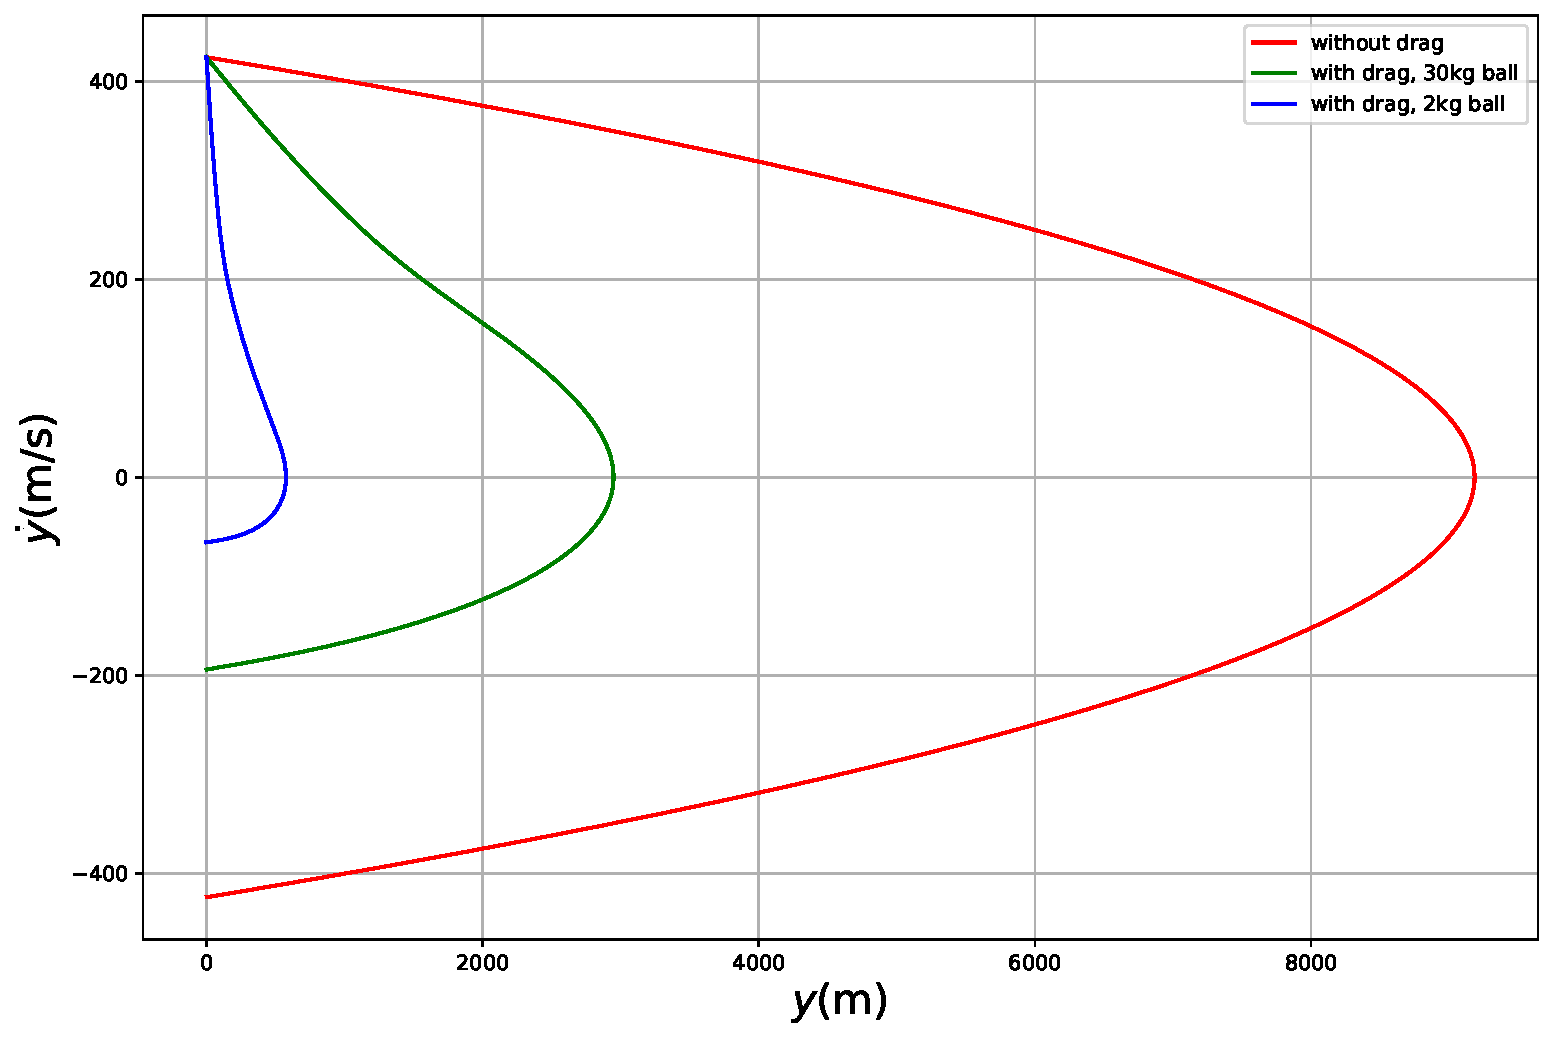
\includegraphics[width=0.87\linewidth]{../figures/yvy}
	\end{figure}
\end{document}
